\documentclass[11pt,twocolumn,oneside,openany,headings=optiontotoc,11pt,numbers=noenddot]{article}

\usepackage[a4paper]{geometry}
\usepackage[utf8]{inputenc}
\usepackage[T1]{fontenc}
\usepackage{lmodern}
\usepackage[ngerman]{babel}
\usepackage{ngerman}

\usepackage[onehalfspacing]{setspace}

\usepackage{fancyhdr}
\usepackage{fancybox}

\usepackage{rotating}
\usepackage{varwidth}

%Struktogramme
\usepackage[german,curves]{struktex}

\usepackage{pdflscape}
\usepackage{changepage}
\usepackage{graphicx}
\usepackage[bottom]{footmisc}
\usepackage{transparent}
\usepackage{graphbox}
\graphicspath{
	{Pics/PDFs/}
	{Pics/JPGs/}
	{Pics/PNGs/}
}
\usepackage{caption}
\usepackage{wrapfig}
\usepackage{marginnote}
\usepackage{tabularx}
\usepackage{dashrule}
\usepackage{soulutf8}
\usepackage{hhline}
%arydshln suppresses vertical lines in table
%\usepackage{arydshln}
\usepackage{multirow}
\usepackage{enumerate}
\usepackage[hidelinks]{hyperref}
\usepackage{listings}

\usepackage[table]{xcolor}
\usepackage{array}
\usepackage{enumitem,amssymb,amsmath}
\usepackage{interval}
\usepackage{cancel}
\usepackage{stmaryrd}
\usepackage{wasysym}
\usepackage{polynom}
\usepackage{diagbox}
\usepackage{dashrule}
\usepackage{framed}
\usepackage{mdframed}
\usepackage{karnaugh-map}
\usepackage{pdfpages}

\usepackage{blindtext}

\usepackage{eso-pic}

\usepackage{amssymb}
\usepackage{eurosym}

\usepackage[pages=some]{background}
\pagestyle{headings}
\renewcommand{\headrulewidth}{0.2pt}
\renewcommand{\footrulewidth}{0.2pt}
\newcommand*{\underdownarrow}[2]{\ensuremath{\underset{\overset{\Big\downarrow}{#2}}{#1}}}
\setlength{\fboxsep}{5pt}
\newcommand{\explainBelow}[3]{\underbrace{#1}_{\parbox{\widthof{#3}}{\footnotesize\raggedright #2}}}
\newcommand{\explainAbove}[3]{\overbrace{#1}^{\parbox{\widthof{#3}}{\footnotesize\raggedright #2}}}
\newcommand\footnoteref[1]{\protected@xdef\@thefnmark{\ref{#1}}\@footnotemark}


% Codestyle defined
\definecolor{codegreen}{rgb}{0,0.6,0}
\definecolor{codegray}{rgb}{0.5,0.5,0.5}
\definecolor{codepurple}{rgb}{0.58,0,0.82}
\definecolor{backcolour}{rgb}{0.95,0.95,0.92}
\definecolor{deepgreen}{rgb}{0,0.5,0}
\definecolor{darkblue}{rgb}{0,0,0.65}
\definecolor{mauve}{rgb}{0.40, 0.19,0.28}
\colorlet{exceptioncolour}{yellow!50!red}
\colorlet{commandcolour}{blue!60!black}
\colorlet{numpycolour}{blue!60!green}
\colorlet{specmethodcolour}{violet}

%Neue Spaltendefinition
\newcolumntype{L}[1]{>{\raggedright\let\newline\\\arraybackslash\hspace{0pt}}m{#1}}
\newcolumntype{M}{>{\centering\arraybackslash}X}
\newcommand{\cmnt}[1]{\ignorespaces}
%Textausrichtung ändern
\newcommand\tabrotate[1]{\rotatebox{90}{\raggedright#1\hspace{\tabcolsep}}}

%Intervall-Konfig
\intervalconfig {
	soft open fences
}

%Bash
\lstdefinestyle{BashInputStyle}{
	language=bash,
	basicstyle=\small\sffamily,
	backgroundcolor=\color{backcolour},
	columns=fullflexible,
	backgroundcolor=\color{backcolour},
	breaklines=true,
}
%Java
\lstdefinestyle{JavaInputStyle}{
	language=Java,
	backgroundcolor=\color{backcolour},
	aboveskip=1mm,
	belowskip=1mm,
	showstringspaces=false,
	columns=flexible,
	basicstyle={\footnotesize\ttfamily},
	numberstyle={\tiny},
	numbers=none,
	keywordstyle=\color{purple},,
	commentstyle=\color{deepgreen},
	stringstyle=\color{blue},
	emph={out},
	emphstyle=\color{darkblue},
	emph={[2]rand},
	emphstyle=[2]\color{specmethodcolour},
	breaklines=true,
	breakatwhitespace=true,
	tabsize=2,
}
%Python
\lstdefinestyle{PythonInputStyle}{
	language=Python,
	alsoletter={1234567890},
	aboveskip=1ex,
	basicstyle=\footnotesize,
	breaklines=true,
	breakatwhitespace= true,
	backgroundcolor=\color{backcolour},
	commentstyle=\color{red},
	otherkeywords={\ , \}, \{, \&,\|},
	emph={and,break,class,continue,def,yield,del,elif,else,%
		except,exec,finally,for,from,global,if,import,in,%
		lambda,not,or,pass,print,raise,return,try,while,assert},
	emphstyle=\color{exceptioncolour},
	emph={[2]True,False,None,min},
	emphstyle=[2]\color{specmethodcolour},
	emph={[3]object,type,isinstance,copy,deepcopy,zip,enumerate,reversed,list,len,dict,tuple,xrange,append,execfile,real,imag,reduce,str,repr},
	emphstyle=[3]\color{commandcolour},
	emph={[4]ode, fsolve, sqrt, exp, sin, cos, arccos, pi,  array, norm, solve, dot, arange, , isscalar, max, sum, flatten, shape, reshape, find, any, all, abs, plot, linspace, legend, quad, polyval,polyfit, hstack, concatenate,vstack,column_stack,empty,zeros,ones,rand,vander,grid,pcolor,eig,eigs,eigvals,svd,qr,tan,det,logspace,roll,mean,cumsum,cumprod,diff,vectorize,lstsq,cla,eye,xlabel,ylabel,squeeze},
	emphstyle=[4]\color{numpycolour},
	emph={[5]__init__,__add__,__mul__,__div__,__sub__,__call__,__getitem__,__setitem__,__eq__,__ne__,__nonzero__,__rmul__,__radd__,__repr__,__str__,__get__,__truediv__,__pow__,__name__,__future__,__all__},
	emphstyle=[5]\color{specmethodcolour},
	emph={[6]assert,range,yield},
	emphstyle=[6]\color{specmethodcolour}\bfseries,
	emph={[7]Exception,NameError,IndexError,SyntaxError,TypeError,ValueError,OverflowError,ZeroDivisionError,KeyboardInterrupt},
	emphstyle=[7]\color{specmethodcolour}\bfseries,
	emph={[8]taster,send,sendMail,capture,check,noMsg,go,move,switch,humTem,ventilate,buzz},
	emphstyle=[8]\color{blue},
	keywordstyle=\color{blue}\bfseries,
	rulecolor=\color{black!40},
	showstringspaces=false,
	stringstyle=\color{deepgreen}
}

\lstset{literate=%
	{Ö}{{\"O}}1
	{Ä}{{\"A}}1
	{Ü}{{\"U}}1
	{ß}{{\ss}}1
	{ü}{{\"u}}1
	{ä}{{\"a}}1
	{ö}{{\"o}}1
}

% Neue Klassenarbeits-Umgebung
\newenvironment{worksheet}[3]
% Begin-Bereich
{
	\newpage
	\sffamily
	\setcounter{page}{1}
	\ClearShipoutPicture
	\AddToShipoutPicture{
		\put(55,761){{
				\mbox{\parbox{385\unitlength}{\tiny \color{codegray}BBS I Mainz, #1 \newline #2
						\newline #3
					}
				}
			}
		}
		\put(455,761){{
				\mbox{\hspace{0.3cm}
\includegraphics[width=0.2\textwidth]{../../logo.pdf}}
			}
		}
	}
}
% End-Bereich
{
	\clearpage
	\ClearShipoutPicture
}

\setlength{\columnsep}{3em}
\setlength{\columnseprule}{0.5pt}

\geometry{left=2.50cm,right=2.50cm,top=3.00cm,bottom=1.00cm,includeheadfoot}
\pagenumbering{gobble}
\pagestyle{empty}

\begin{document}
	\begin{worksheet}{Berufliches Gymnasium}{Klassenstufe 13 - Mathematik}{Lernabschnitt 1: Wiederholung Kurvendiskussion}
		\section{Die Kurvendiskussion}
		Vor geraumer Zeit haben wir uns mit Funktionen und der Untersuchung ebendieser beschäftigt. Wir erinnern uns noch, dass Funktionen verwendet werden um Entwicklungen bzw. Zusammenhänge zu modellieren.\\
		Unser Gehirn verlegt aber bekanntlich unnötige Informationen in die hinterste Ecke. Daher nachfolgend nochmal eine kurze Auffrischung zur Kurvendiskussion.
		\subsection{Das Ziel}
		Bei der Kurvendiskussion wollen wir die charakteristischen Merkmale einer Funktion bestimmen, um mit diesen Informationen die modellierten Zusammenhänge bzw. die Entwicklungen in einem Graph darzustellen, zu analysieren und zu interpretieren.
		\subsection{Die Methodik}
		Um also die charakteristischen Merkmale herauszuarbeiten, machen wir uns die bekannten Zusammenhänge zwischen dem Funktionsterm und dem Graph zunutze.\\
		Besonderen Nutzen können wir aber von den Zusammenhängen zwischen der Funktion und ihren Ableitungsfunktionen ziehen.
		\section{Rund um die Ableitung}
		\subsection{Die Ableitung der Stelle}
		Ganz klar ist, wir benötigen den Funktionswert an einer Stelle um den Graphen skizzieren zu können. Manchmal ist es aber auch hilfreich die Steigung an genau diesem Punkt zu kennen.\\
		\par\bigskip\noindent
		\textit{Wir betrachten die Funktion \(y=-0,1x^2+1,2x+2,4\). Sie modelliert die Entwicklung der Anmeldungen von Kindern in Kindertagesstätten in Kiel (x: in Jahren, 0 = 2010, y: Anzahl Kinder)}\\
		\par\bigskip\noindent
		\begin{tabularx}{0.5\textwidth}{X|X|}
			\cline{2-2}
			\multirow{2}{*}{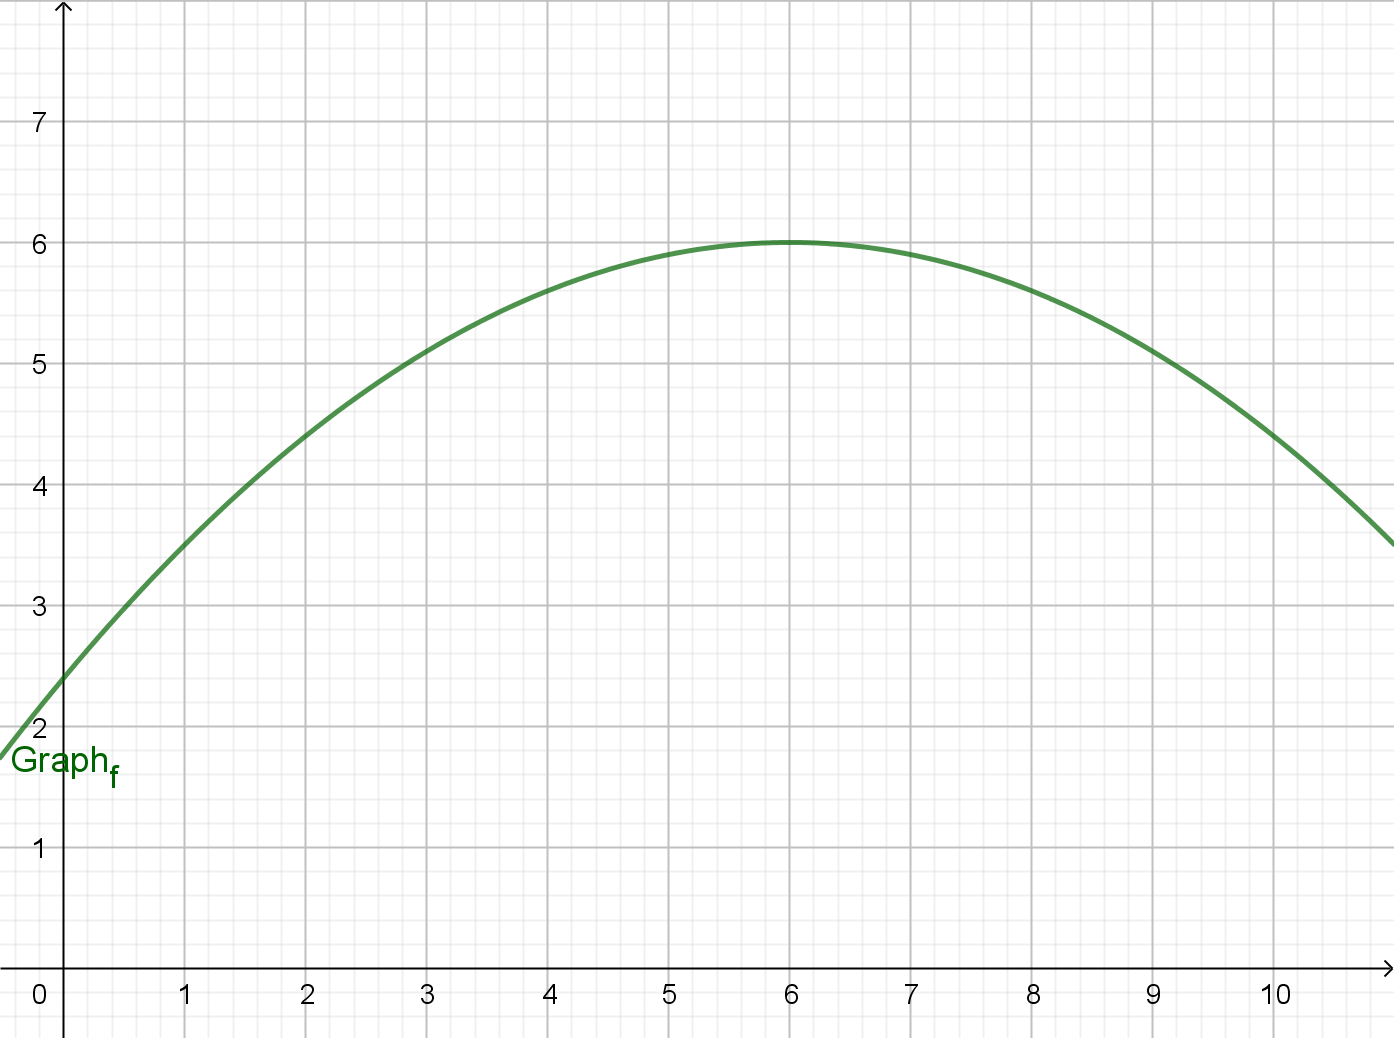
\includegraphics[align=t,width=0.23\textwidth]{../99_Bilder/00_Wdh/KiTa.png}} &
			Die Stadtverwaltung kann erkennen, dass \textit{2014} insgesamt \textbf{5.600 Kinder} zu betreuen waren.\\
			& Für eine bessere Planung wüssten sie aber gerne auch, wie die momentane Wachstumstendenz in diesem Jahr ist.\\
			\cline{2-2}
		\end{tabularx}
		\par\bigskip\noindent
		Wir erinnern uns, dass sich die momentane Wachstumstendenz als Steigung der Tangente durch den entsprechenden Punkt verstehen lässt. Wir legen also eine Tangente an den Punkt.\\
		\par\bigskip\noindent
		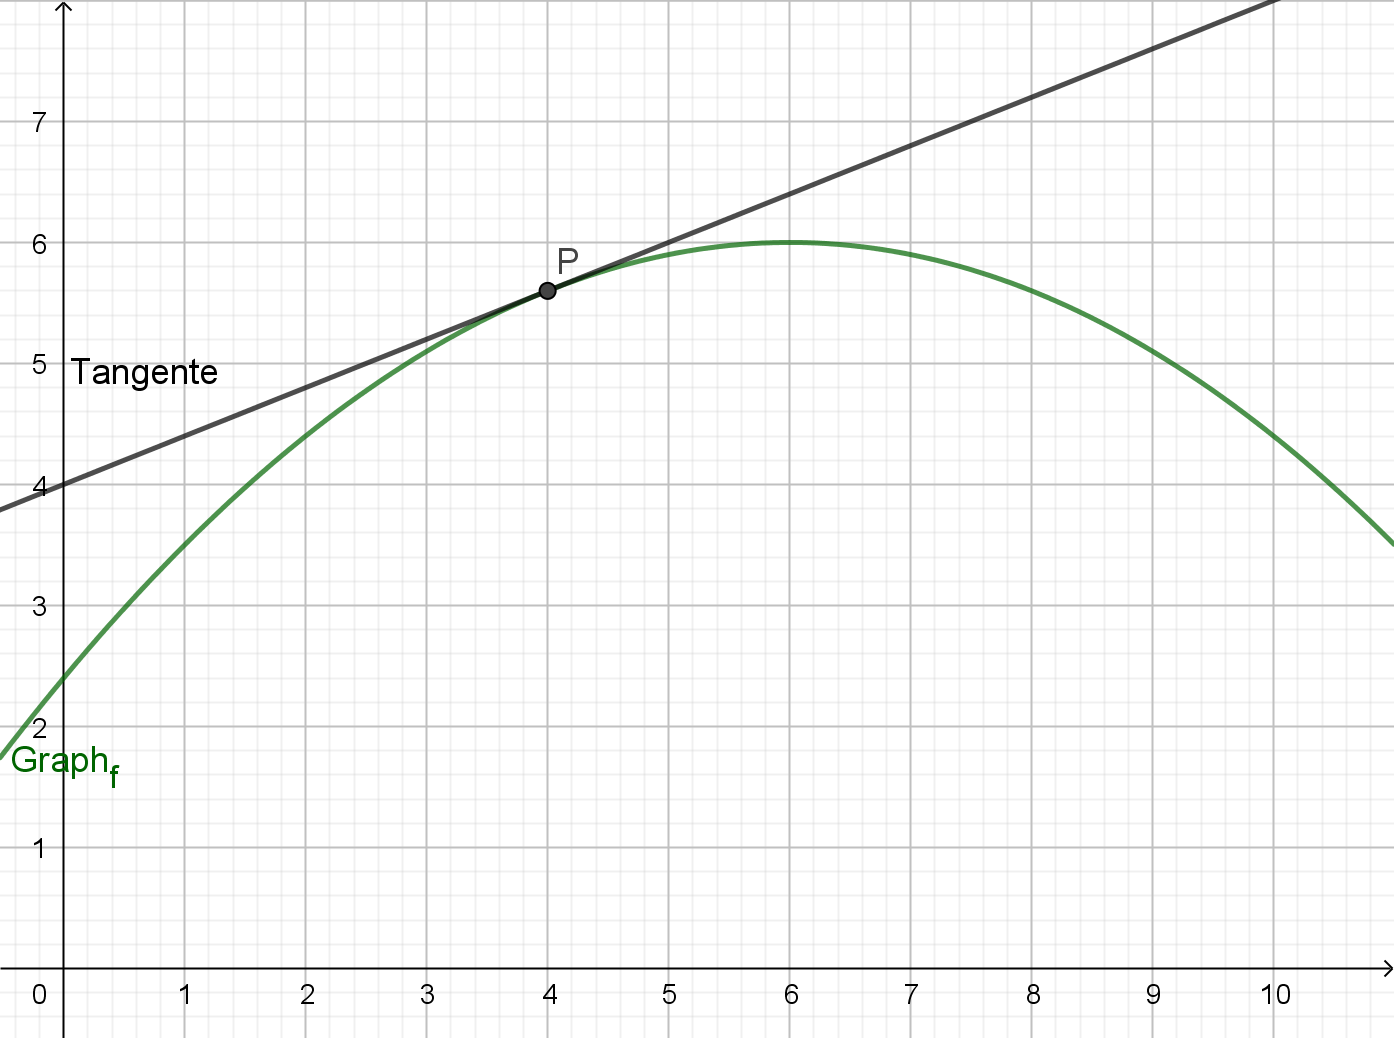
\includegraphics[width=0.48\textwidth]{../99_Bilder/00_Wdh/KiTa1.png}\\
		\par\bigskip\noindent
		Schauen wir uns die Tangente in dem Punkt genauer an, können wir mittels dem Steigungsdreieck die Steigung der Tangente und somit die Steigung des Graphen in diesem Punkt ermitteln.\\
		\par\bigskip\noindent
		\begin{tabularx}{0.48\textwidth}{X}
			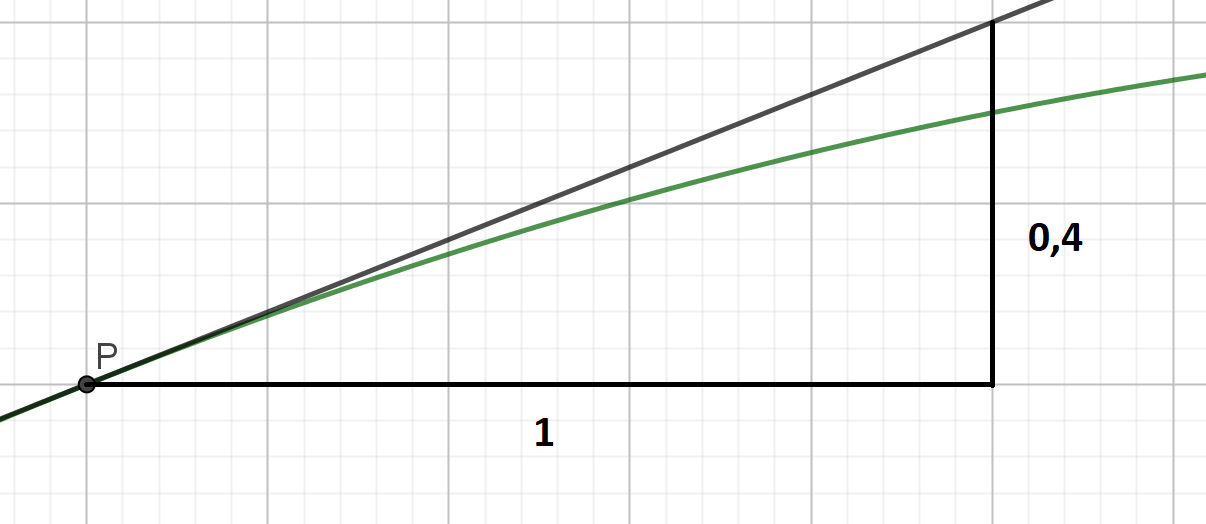
\includegraphics[width=0.48\textwidth]{../99_Bilder/00_Wdh/KiTa2.png}\\
			Die Steigung der Tangente lässt sich durch die Seitenlängen das Steigungsdreieck ermitteln: \(\frac{\Delta{}y}{\Delta{}x}= \frac{0,4}{1} = 0,4\)\\
			Daraus können wir Schlussfolgern, dass die momentane Wachstumstendenz bei \textbf{400 Kindern} pro Jahr liegt.\\
		\end{tabularx}
		\par\bigskip\noindent
		\textit{Welche Schlussfolgerung können Sie daraus ziehen?}\\
		\par\bigskip\noindent
		\begin{framed}
			Die Einheit des Ableitungswerts ist die Bedeutung einer Einheit auf der y-Achse geteilt durch die Bedeutung einer Einheit auf der x-Achse. Ein Ableitungswert bei einer Zeitreihe bedeutet also die momentane Änderungsdynamik zum Zeitpunkt x in \glqq{}Einheit auf der y-Achse\grqq{} pro \glqq{}Zeiteinheit auf der x-Achse\grqq{}.
		\end{framed}
		\subsection{Die Ableitungsfunktion}
		Wir erinnern uns noch dunkel daran, dass jede Funktion \(f\) eine passende Ableitungsfunktion \(f'\) besitzt. Diese gibt uns für jede Stelle den Wert der Ableitung an.\\
		Bei ganzrationalen Funktionen kann man die Gleichung durch die Ableitungsregeln bestimmen: \(f(x) = a\cdot{}x^n\rightarrow{}f'(x) = a\cdot{}n\cdot{}x^{n-1}\)\\
		\par\bigskip\noindent
		\textit{Schauen wir uns die Funktion \(f(x) = -0,1x^2 + 1,2x +2,4\) und deren Ableitungsfunktion aus dem letzten Beispiel an. Die Ableitungsfunktion hat laut obiger Regel die Form \(f'(x) = -0,2x + 1,2\)}. Dementsprechend sieht der Graph dann so aus:\\
		\par\bigskip\noindent
		\begin{tabularx}{0.5\textwidth}{X}
			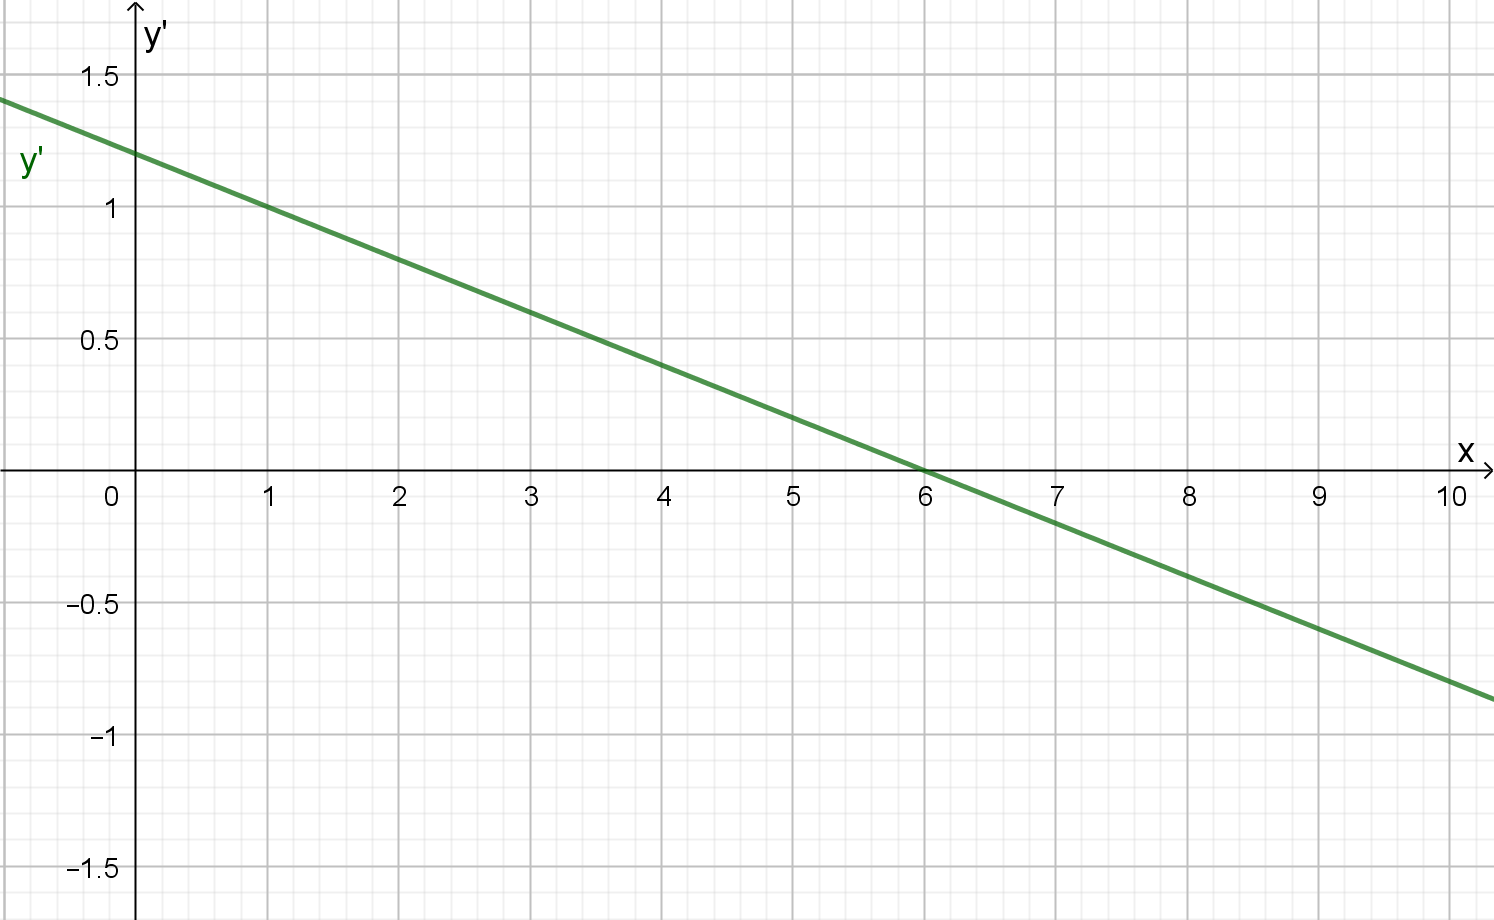
\includegraphics[width=0.48\textwidth]{../99_Bilder/00_Wdh/KiTa'.png}\\
			\\
			\textit{Am Graphen können wir ablesen, dass die Ableitungsfunktion für \(x=4\) den Wer \(f'(4)=0,4\) hat.}
			\textit{\textbf{Außerdem} können wir ablesen, dass die Funktion an der Stelle \(x=6\) eine \underline{Extremstelle} vom Typ \underline{Hochpunkt} besitzt.}
		\end{tabularx}
		\subsection{Zusammenhänge zwischen Funktion und Ableitungsfunktion}
		\label{zsmhg}
		Um das alter Wissen noch einmal aufzufrischen und eine Übersicht zu haben, finden Sie in der nachfolgenden Tabelle die entsprechenden Zusammenhänge mit einer kurzen Erläuterung.\\
		\newpage
		\setlength{\columnseprule}{0pt}
		\begin{tabularx}{\textwidth}{|X|X|X|X|}
			\multicolumn{1}{X|}{}& 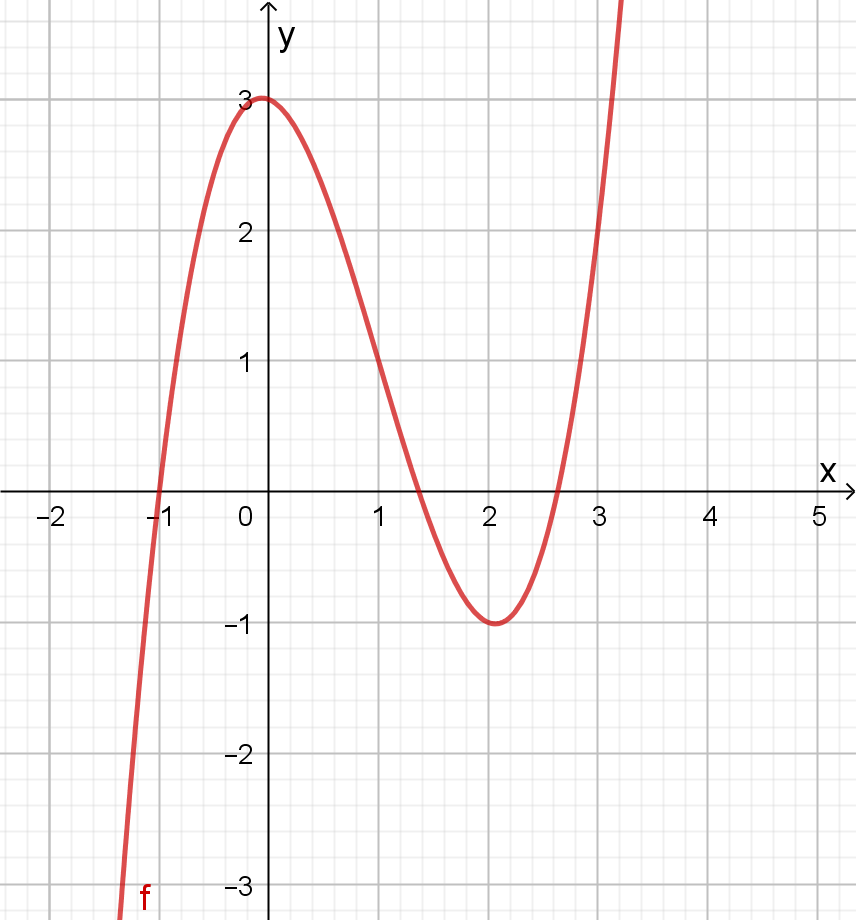
\includegraphics[width=0.15\textwidth]{../99_Bilder/00_Wdh/Bsp.png} & 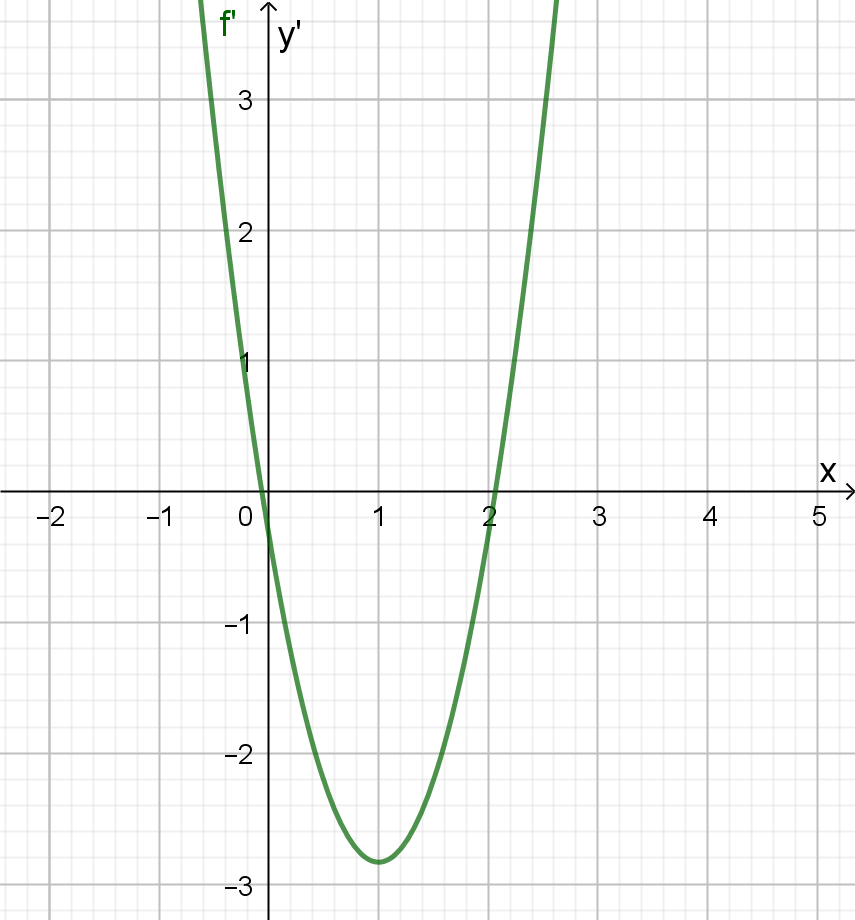
\includegraphics[width=0.15\textwidth]{../99_Bilder/00_Wdh/Bsp'.png} & 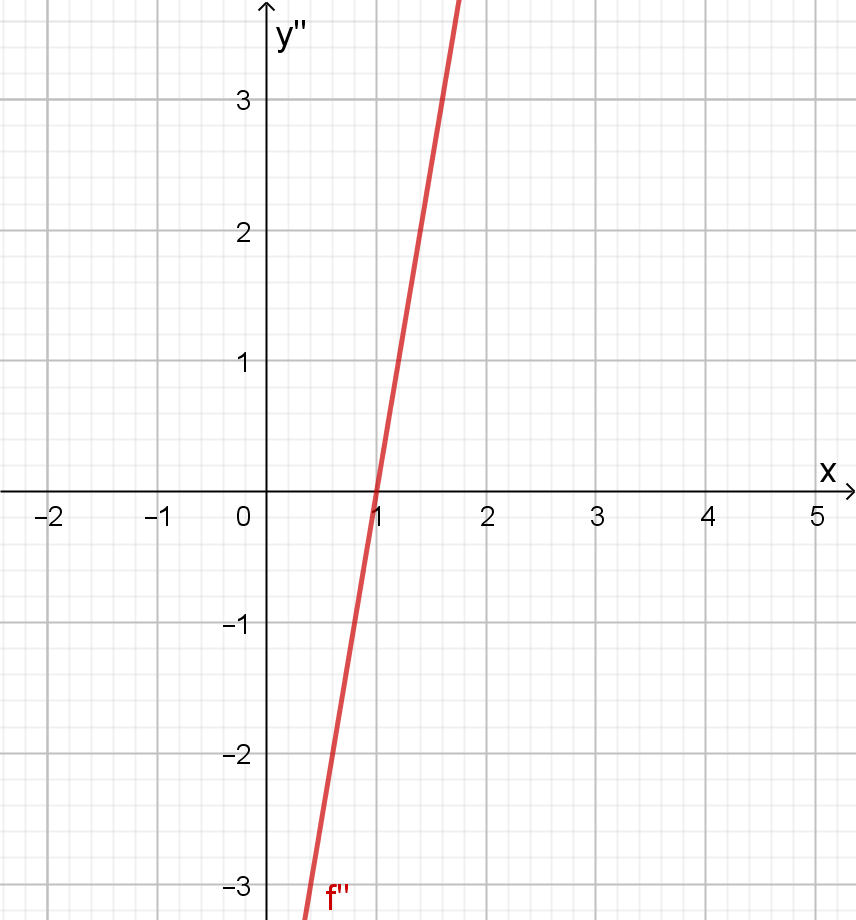
\includegraphics[width=0.15\textwidth]{../99_Bilder/00_Wdh/Bsp''.png}\\
			\hline
			\hline
			\textbf{Extremstelle Typ Hochpunkt bei \(x_{HP}\)} & Punkt mit \underline{höchstem} Funktionswert für eine Umgebung von \(x_{HP}\) & Nullstelle bei \(x_{HP}\) - (\(f'(x_{HP}) = 0\)) und Ableitungsgraph ist fallend an der Stelle \(x_{HP}\) & \(f''(x_{HP}) < 0\)\\
			\hline
			\textbf{Extremstelle Typ Tiefpunkt bei \(x_{TP}\)} & Punkt mit \underline{niedrigstem} Funktionswert für eine Umgebung von \(x_{TP}\) & Nullstelle bei \(x_{TP}\) - (\(f'(x_{TP}) = 0\)) und Ableitungsgraph ist an der Stelle \(x_{TP}\) steigend & \(f''(x_{TP}) < 0\)\\
			\hline
			\textbf{Sattelstelle bei \(x_{SP}\)} & Wechsel im Krümmungsverhalten, \underline{kein Wechsel} im Steigungsverhalten & \underline{Doppelte} Nullstelle bei \(x_{SP}\) & Nullstelle bei \(x_{SP}\)\\
			& & \(f'(x_{SP}) = 0\) & \(f''(x_{SP}) = 0\)\\
			\hline
			\textbf{Fallend über Intervall \([a;b]\)} & Für alle \(x_0, x_1\) aus \([a,b]\) gilt: & Graph verläuft unterhalb der x-Achse & \\
			& Wenn \(x_0 < x_1\) dann ist & \(f'(x) < 0\) & \\
			& \(f(x_0) > f(x_1)\) & & \\
			\hline
			\textbf{Steigend über Intervall \([a;b]\)} & Für alle \(x_0, x_1\) aus \([a,b]\) gilt: & Graph verläuft oberhalb der x-Achse &\\
			& Wenn \(x_0 < x_1\) dann ist & \(f'(x) > 0\) & \\
			& \(f(x_0) < f(x_1)\) & & \\
			\hline
			\textbf{Wendepunkt bei \(x_{WP}\)} & Wechsel beim Krümmungsverhalten & Punkt mit höchstem/niedrigsten Ableitungswert \(f(x_{WP})'\) für eine Umgebung von \(x_{WP}\) & Nullstelle bei \(x_0\)\\
			& & & \(f''(x_0) = 0\)\\
			\hline
		\end{tabularx}
		\par\bigskip\noindent
		\clearpage
		\setlength{\columnseprule}{0.1pt}
		\section{Elemente der Kurvendiskussion}
		Bei einer solchen Kurvendiskussion untersucht man die Funktion und deren Ableitungen auf besondere Charakteristika. Im nachfolgenden werden die Informationen und Charakteristika kurz beleuchtet, die dabei die größte Relevanz haben.
		\subsection{Definitionsbereich}
		Als \textbf{Definitionsbereich} einer Funktion \(f\) bezeichnet man alle Zahlen, mit denen man \(x\) besetzen kann, ohne dass gegen bekannte Rechenregeln (\textit{z.B. 0 im Nenner, Wurzel einer negativen Zahl}) verstoßen wird.\\
		\textit{\underline{Beispiel:} Betrachten wir die Funktion \(f(x) = \frac{1}{x}\). Der Definitionsbereich entspricht also \(\mathbb{D} = \mathbb{R}\setminus\{0\}\) (Alle reellen Zahlen außer die Null).}
		\subsection{y-Achsenabschnitt}
		Eine andere Bezeichnung für \textbf{y-Achsenabschnitt} ist auch \underline{Schnittpunkt mit der y-Achse}.\\
		Das bedeutet also, wir bestimmen den y-Achsenabschnitt einer Funktion indem wir \(x=0\) setzen und damit den Funktionswert \(f(0) = y\) zu dieser Stelle berechnen.\\
		\textit{\underline{Beispiel:} Sei \(y = f(x) = x^3 +3x^2 -3\). Dann entspricht der y-Achsenabschnitt dem Wert \(-3\), da \(f(0) = 0^2 +3\cdot{}0^2 -3 = -3\).}
		\begin{framed}
			\noindent
			Angenommen die Funktion modelliert die Entwicklung einer Größe (y) (z.B. Aktienwert) über mehrere Jahre (x), so entspricht der \underline{y-Achsenabschnitt} dem Wert zum Zeitpunkt 0.
		\end{framed}
		\subsection{Nullstellen}
		\label{nst}
		Als \textbf{Nullstelle} bezeichnen wir den \underline{Schnittpunkt mit der x-Achse}. Somit wird zur Berechnung der Nullstelle \(y = f(x) = 0\) gesetzt und anschließend wird diese Gleichung gelöst, um die passende x-Besetzung zu bestimmen.\\
		Um diese Gleichungen zu lösen kennen wir verschiedene Verfahren. Die, die am wertvollsten sind, sind \glqq{}Faktorisieren\grqq{} sowie die Anwendung der \glqq{}pq-Formel\grqq{}.\\
		\par\noindent
		\textit{\underline{Beispiel:}}
		\begin{align*}
			f(x) & = x^3-2x\\
			0 & = x^3 -2x\\
			0 & = x^2(x-2)\\
			& \Rightarrow x^2 = 0\ \ \Rightarrow x_{1,2} = 0\\
			& \text{(Es handelt sich um eine \underline{doppelte Nullstelle}.}\\ & \text{Also berührt der Graph die x-Achse, er}\\
			& \text{schneidet sie aber nicht.)}\\
			oder & \Rightarrow x-2 = 0\ \ \Rightarrow x_3 = 2\\
			& \text{(einfache Nullstelle)}
		\end{align*}
		\begin{framed}
			\noindent
			Stellt unser Graph die Entwicklung einer Größe (y) (\textit{z.B. Bevölkerungszahl}) über eine bestimmte Zeit (x) dar, so entspricht die \underline{Nullstelle} dem Zeitpunkt, an dem das \glqq{}Niveau 0\grqq{} bzw. der Ausgangswert erreicht wird. Hierbei geht der Wert dieses \glqq{}Niveau 0\grqq{} aus der Skalierung der y-Achse hervor (\textit{z.B. y: 0 = Stand 1990 \(\rightarrow\) 3,4 Mio.})
		\end{framed}
		\par\noindent
		\subsection{Extremstellen - relative Minima/Maxima und Sattelstelle}
		Als \textbf{Extremstelle} \(\mathbf{x_E}\) bezeichnen wir die Stellen, bei denen die Funktion ein relatives Maximum (Extremstelle vom \underline{Typ Hochpunkt}) oder relatives Minimum (Extremstelle vom \underline{Typ Tiefpunkt}) hat.\\
		Als \textbf{relatives Maximum} bzw. \textbf{relatives Minimum} wird der Wert \(x_E\) bezeichnet, der für eine bestimmte Umgebung der \underline{höchste} bzw. \underline{niedrigste} ist.\\
		Logischerweise ist der Graph zwischen zwei Extremstellen entweder \textbf{monoton fallend} bzw. \textbf{monoton steigend}.\\
		\par\bigskip\noindent
		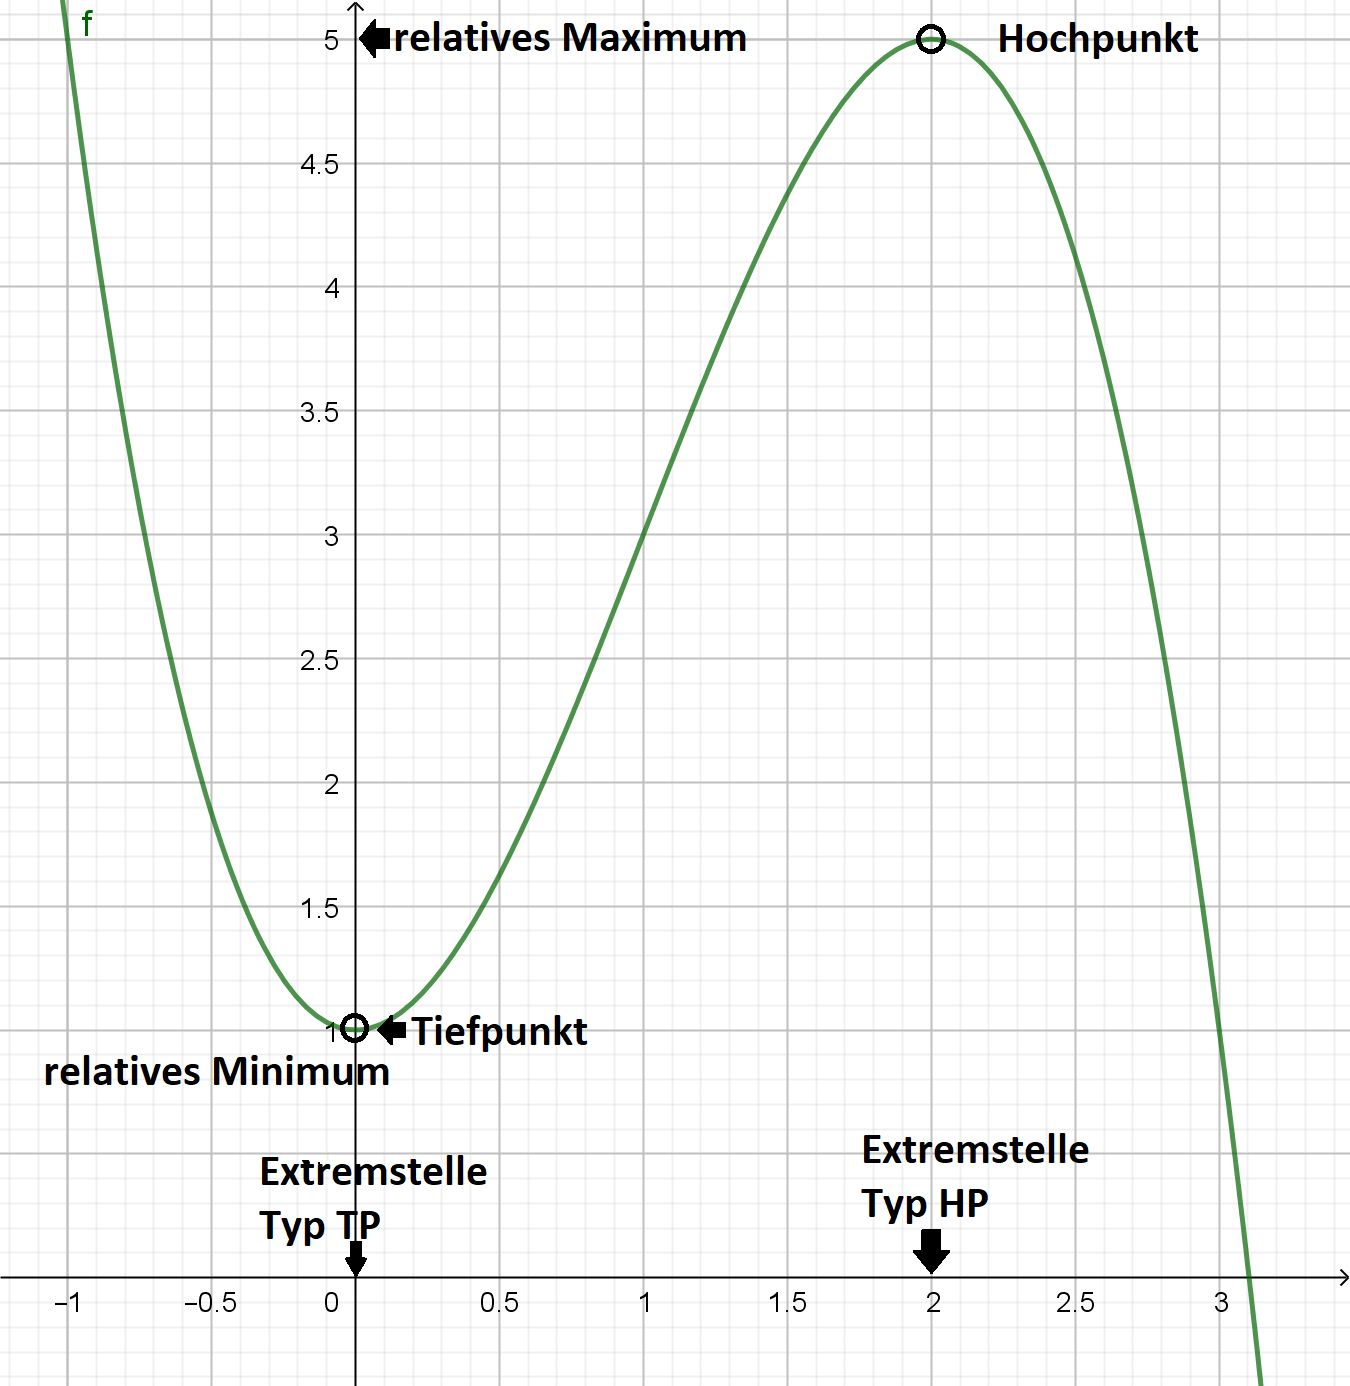
\includegraphics[width=0.48\textwidth]{../99_Bilder/00_Wdh/EP.png}\\
		\par\bigskip\noindent
		Um die Extremstelle zu berechnen, bestimmt man die Nullstellen (\ref{nst}) der ersten Ableitungsfunktion bestimmt. Mit dem Wert der zweiten Ableitung an bestimmter Extremstelle lässt sich schlussfolgern, um welchen Typ von Extremstelle es sich handelt bzw. ob es sich möglicherweise um eine Sattelstelle handelt.\\
		\textit{Beispielrechnung:}
		\begin{align*}
			f(x) & = x^3 - 3x^2 +3\\
			f'(x) & = 3x^2 - 3x\\
			0 & = 3x^2 - 6x\\
		\end{align*}
		\begin{align*}
			0 & = 3x(x-2)\\
			x_1 & = 0\ \ \ x_2=2\ \ (\text{Kandidaten für Extrem-}\\
			& \text{stellen})
		\end{align*}
		\textit{Zur Bestimmung des Typs der Extremstelle (also HP, TP oder SP(eine Extremstelle)):}
		\begin{align*}
			f''(x) & = 6x - 6\\
			f''(0) & = 6\cdot{}0 - 6 = -6\\
			& \rightarrow \mathbf{Extremstelle\ vom\ Typ}\\
			& \mathbf{Hochpunkt\ bei\ } x = 0\\
			f''(2) & = 6\cdot{}2 - 6 = 6\\
			& \rightarrow \mathbf{Extremstelle\ vom\ Typ}\\
			& \mathbf{Tiefpunkt\ bei\ } x = 6\\
		\end{align*}
		Beachte: wenn \(f''(x) = 0\) handelt es sich bei x möglicherweise um eine Sattelstelle.\\
		\par\bigskip\noindent
		Abschließend berechnen wir die zugehörigen relativen Minima/Maxima:
		\begin{align*}
			\text{Relatives Maximum: } f(0) & = 0^3 -3\cdot{}0^2 + 3 = 3\\
			& \rightarrow\ \text{Hochpunkt (0|3)}\\
			\text{Relatives Minimum: } f(2) & = 2^3 -3\cdot{}2^2 + 3 = -1\\
			& \rightarrow\ \text{Tiefpunkt (2|-1)}
		\end{align*}
		\begin{framed}
			\noindent
			Bei einer Funktion geben die \underline{Extremstellen} die Zeitpunkte an, bei denen ein niedrigster oder ein höchster Wert für einen gewissen Zeitraum vor und nach diesem Zeitpunkt erreicht wurde.\\
			Das \underline{relative Maximum} bzw. \underline{Minimum} gibt dann das höchste bzw. niedrigste Niveau für einen bestimmen Zeitraum um die Extremstelle an.
		\end{framed}
		\subsection{Wendestelle}
		An der \textbf{Wendestelle} findet beim Funktionsgraph eine Änderung des Krümmungsverhaltens statt.\\
		\par\bigskip\noindent
		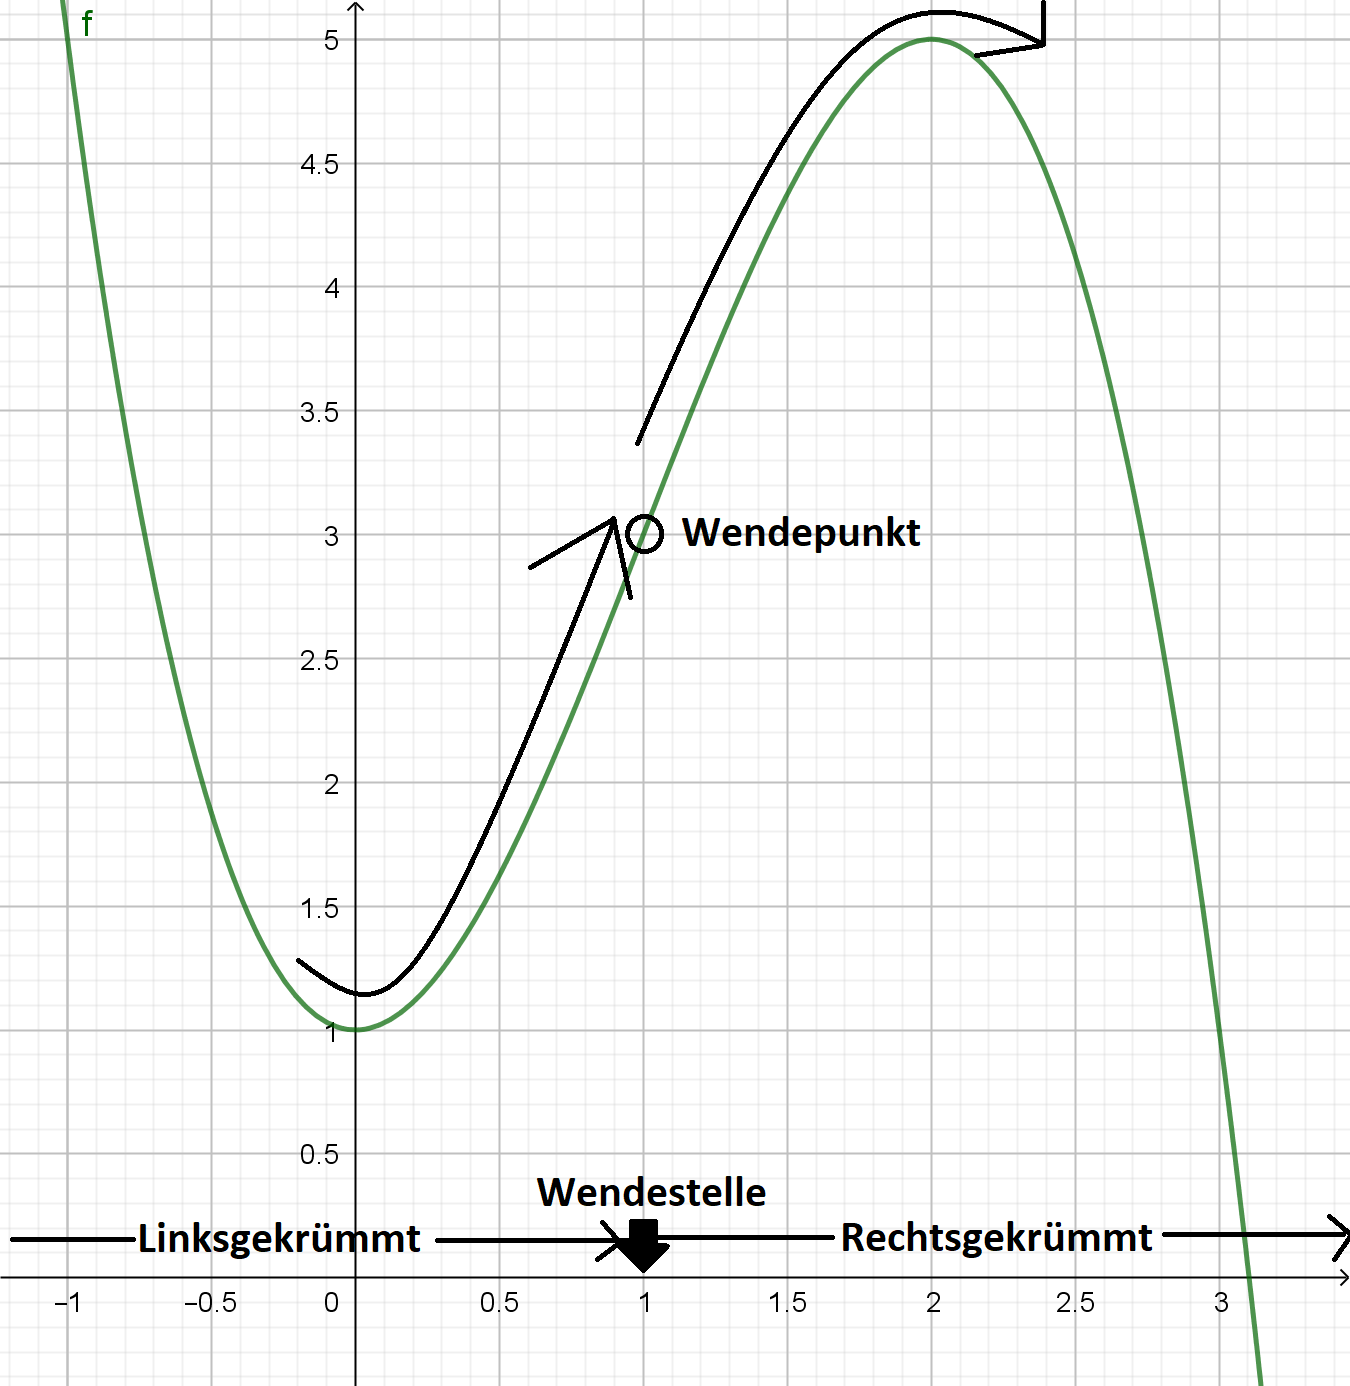
\includegraphics[width=0.48\textwidth]{../99_Bilder/00_Wdh/WP.png}\\
		par\bigskip\noindent
		Um die Wendestellen zu berechnen, bestimmt man die Nullstellen der zweiten Ableitungsfunktion.\\
		\textit{\underline{Beispiel:}} \(f(x) = x^3 - 3x^2 + 3\)
		\begin{align*}
			f''(x) & = 6x - 6\\
			0 & = 6x - 6\\
			6 & = 6x\\
			\Rightarrow x & = 1
		\end{align*}
		\begin{framed}
			\noindent
			Anders formuliert kann man sagen, dass die \underline{Wendestelle} den Zeitpunkt angibt, an die die Dynamik oder das Wachstum am \textit{höchsten} oder \textit{niedrigsten} für einen gewissen Zeitraum vor und nach diesem Zeitpunkt.\\
			Wir können uns merken, dass der Anstieg bzw. Abfall nach einer Wendestelle stärker oder schwächer wird.
		\end{framed}
		\subsection{Verhalten für große x-Beträge - Grenzwert}
		Wichtig ist noch zu wissen, wo der Graph herkommt und wohin er verläuft. Dieses Verhalten der Funktionswerte für große x-Beträge wird durch die Symbolik \(f(x) \xrightarrow{x\rightarrow-\infty} \ldots\) bzw. \(f(x) \xrightarrow{x\rightarrow\infty} \ldots\) ausgedrückt.\\
		Hierbei ist es möglich, dass sich die Funktionswerte entweder einer bestimmten Zahl annähern oder aber beliebig groß bzw. klein werden.\\
		Nähern sich die Funktionswerte einer bestimmten Zahl an, so nennt man diese Zahl \textbf{Grenzwert} der Funktion.\\
		\textit{\underline{Beispiel:} Betrachten wir die Funktion \(f(x) = \frac{1}{x}\). Das Verhalten dieser Funktion lässt sich wie folgt ausdrücken:}\\
		\par\noindent
		\begin{tabularx}{0.5\textwidth}{c|c}
			\(f(x)\xrightarrow{x\rightarrow-\infty}0\) & \(f(x)\xrightarrow{x\rightarrow\infty}0\)\\
			\multicolumn{1}{c|}{oder} & \multicolumn{1}{c}{oder}\\
			\(\lim\limits_{x\rightarrow-\infty}f(x) = 0\) & \(\lim\limits_{x\rightarrow\infty}f(x) = 0\)
		\end{tabularx}
		\par\bigskip\noindent
		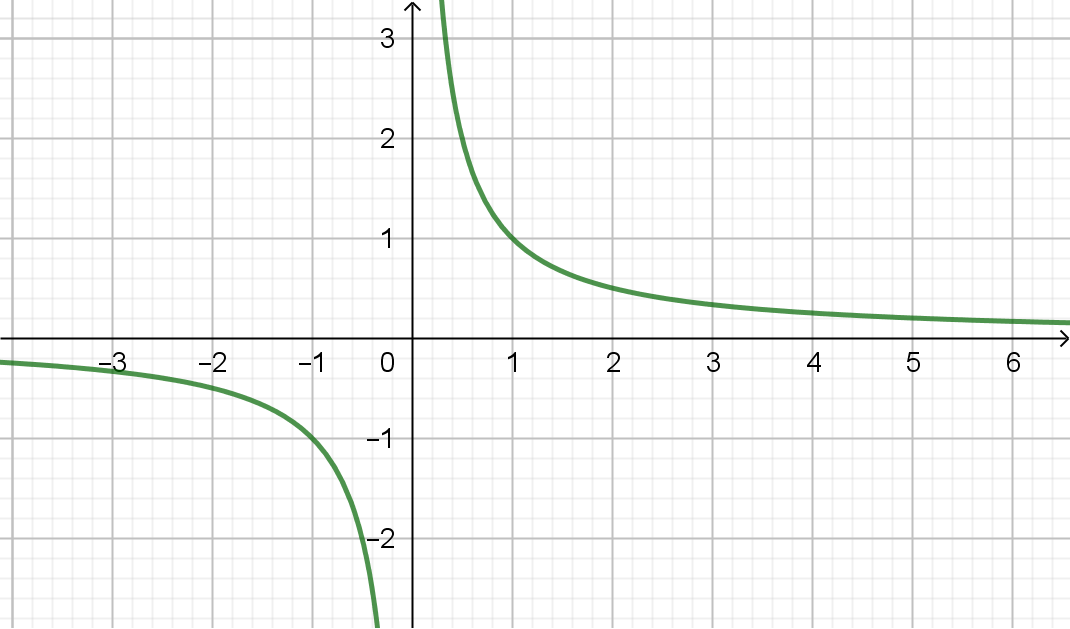
\includegraphics[width=0.48\textwidth]{../99_Bilder/00_Wdh/gw.png}
		\section{Parameter in einer Funktionsgleichung}
		Bisher haben wir uns nur mit Funktionen beschäftigt, die lediglich \(x\) als \textit{Variable} beinhalten.\\
		Es ist aber auch möglich, dass zusätzlich zu Zahlen und \textit{Variablen} \glqq{}x\grqq{} auch weitere Buchstaben (häufig \glqq{}t\grqq{} oder \glqq{}a\grqq{}) auftauchen - \textit{z.B. \(f(x) = x^3 - tx^2\)}. Diese Buchstaben bezeichnet man als \textbf{Parameter}.\\
		Bei Parametern gilt dann, dass jede Besetzung von t eine eigene Funktion definiert. Nimmt man alle so definierten Funktionen zusammen, so erhält man eine \textbf{Funktionsschar}, welche durch eine \underline{Graphenschar} dargestellt werden kann.\\
		\par\noindent
		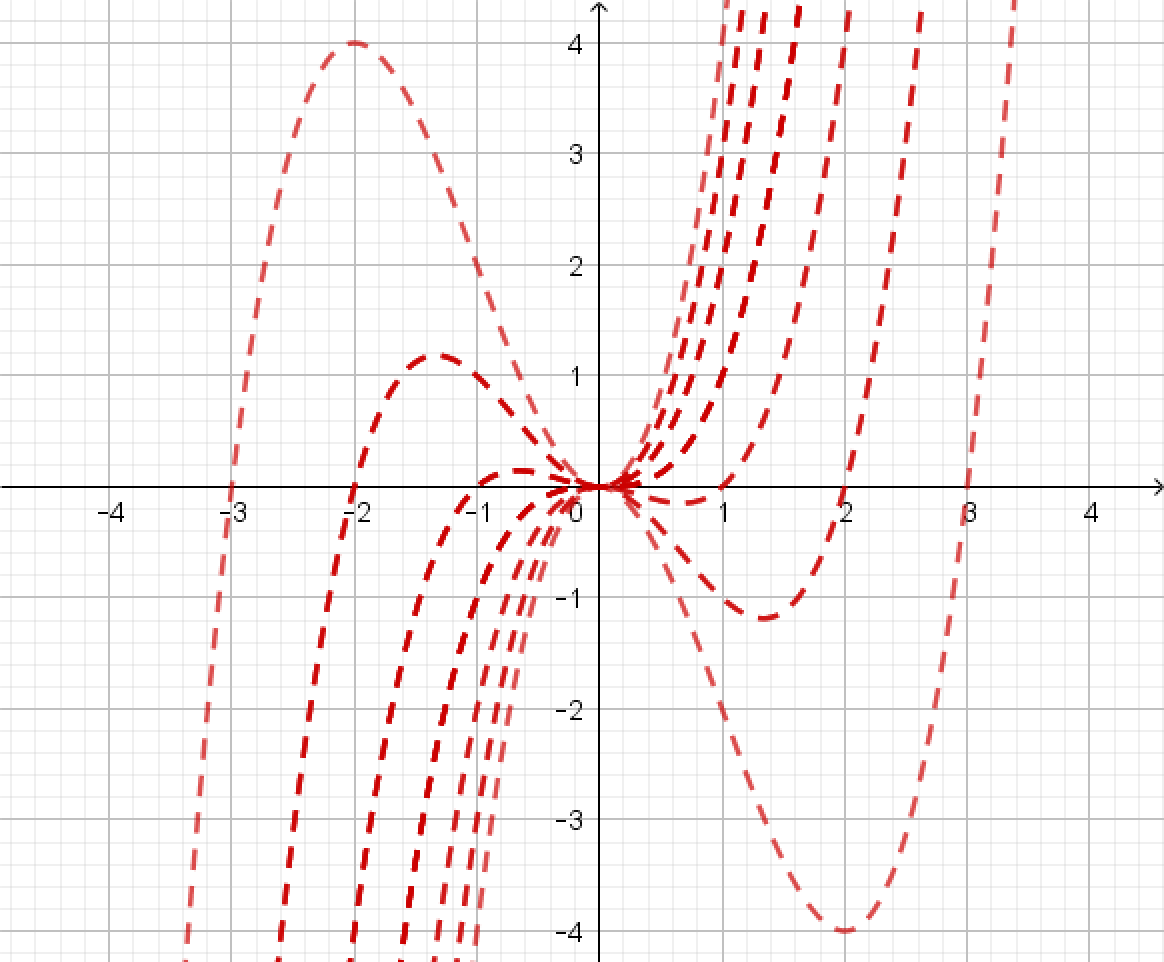
\includegraphics[width=0.48\textwidth]{../99_Bilder/00_Wdh/fSchr.png}\\
		Untersucht man die Funktionsschar, führt also eine Kurvendiskussion durch, zählt der Parameter als eigene feste Zahl. Er kann im Gegensatz zu den anderen Zahlen nicht verrechnet werden.\\
		Das heißt, bei der Berechnung einer Extremstelle erhält man diese in Abhängigkeit des Parameters.\\
		\textit{\underline{Beispiel:} \(f'(x) = 3x^2 -2tx\)}
		\begin{align*}
			0 & = 3x^2 - 2tx\\
			0 & = x(3x - 2t)\\
			x_1 & = 0\\
			\\
			3x - 2t & = 0\\
			3x & = 2t\\
			x_2 & = 0,67t
		\end{align*}
	\end{worksheet}
\end{document}